\documentclass[a4paper, 12pt]{article}
\usepackage[brazil]{babel}
\usepackage[utf8]{inputenc}
\usepackage{amsmath}
\usepackage{indentfirst}
\usepackage{graphicx}
\usepackage{multicol,lipsum}
\usepackage{cite}
\usepackage{placeins}
\usepackage{amsmath,amssymb,amsfonts}
\usepackage{algorithmic}
\usepackage{graphicx}
\usepackage{float}
\usepackage{textcomp}
\usepackage{xcolor}
\usepackage{subfigure}
\usepackage{enumerate}
\usepackage{wrapfig}
\usepackage{cite}
\usepackage{tikz}
\hfuzz=66.002pt

\usepackage{listings}
\usepackage{color}
 
\definecolor{codegreen}{rgb}{0,0.6,0}
\definecolor{codegray}{rgb}{0.5,0.5,0.5}
\definecolor{codepurple}{rgb}{0.58,0,0.82}
\definecolor{backcolour}{rgb}{0.95,0.95,0.92}

\lstdefinestyle{mystyle}{
    backgroundcolor=\color{backcolour},   
    commentstyle=\color{codegreen},
    keywordstyle=\color{magenta},
    numberstyle=\tiny\color{codegray},
    stringstyle=\color{codepurple},
    basicstyle=\footnotesize,
    breakatwhitespace=false,         
    breaklines=true,                 
    captionpos=b,                    
    keepspaces=true,                 
    numbers=left,                    
    numbersep=5pt,                  
    showspaces=false,                
    showstringspaces=false,
    showtabs=false,                  
    tabsize=2
}

\lstset{style=mystyle}

\begin{document}
\begin{titlepage}
    \begin{center}
		\LARGE{Universidade Federal de Mato Grosso do Sul}\\
		\vspace{15pt}
        \large{Campus Ponta Porã}\\ 
        \large{{\textbf{Análise de Algoritmos I}}}\\ 
        \vspace{15pt}
        \vspace{95pt}
        \textbf{\large{Trabalho Prático I}}\\
        \vspace{15pt}
        \textbf{\LARGE{Análise Assintótica}}\\
        %\title{{\large{Título}}}
        \vspace{3,5cm}
    \end{center}
    
    \begin{flushleft}
        \begin{tabbing}
            Aluno: Daniel de Leon Bailo da Silva\\
            Professor: Eduardo Theodoro Bogue\\
            %Professor co-orientador: \\
    \end{tabbing}
 \end{flushleft}
    \vspace{1cm}
    
    \begin{center}
        \vspace{\fill}
             Abril\\
         2019
            \end{center}
\end{titlepage}

\newpage
\tableofcontents
\thispagestyle{empty}

% % % % % % % % % % % % % % % % % % % % % % % % % % %
\newpage
\pagenumbering{arabic}
\section{Resumo}
\newpage

\section{Fibonacci Recursivo}

\begin{lstlisting}[language=Python, caption= Código da função do Fibonacci Recursivo]
def fib(n):
	if n==1 or n==2:
		return 1
	return fib(n-1)+fib(n-2)
\end{lstlisting}

Temos que a recorrência do Fibonacci Recursivo pode ser escrita como:
\begin{equation}
T(n) = \left\{ \begin{array}{l}
O(1), n=0, n=1 \\
fib(n-1)+fib(n-2), n>1\\
\end{array}
\right.
\end{equation} \\

\large\underline{\bf Número de operações} \\

se $n = 0, n = 1$\\
Temos que o número de operações é igual a $fib(n) = 2$

se $n>1$\\
Temos que o número de operações é igual a $fib(n) = 2$ \\

\begin{tikzpicture}
\tikzstyle{level 1} = [sibling distance = 4cm]
\tikzstyle{level 2} = []%\tikzstyle{level 3} = [sibling distance = 6cm,level distance = 4cm]
%

	\node{$fib(n) = 2$}
		child{
			node{$fib(n-1) = 2$}
			child{node{$fib(n-2) = 2$}}
			child{node{$fib(n-3) = 2$}}
		}
		child{
			node{$fib(n-2) = 2$}
		}
	;
\end{tikzpicture} \\

E assim sucessivamente até chegar no caso base. Temos que essa árvore, sempre crescerá mais para a esquerda. No pior caso, teremos que a cada nível da árvore, o número de operações é multiplicado por 2. Pois, cada nó terá dois filhos, e cada filho gasta 2 operações. Ou seja, podemos representar o custo por nível como: \\
$\{2,4,8,16,32,64,...\}$ \\

E que o tamanho dessa sequência, depende do $n$ escolhido, temos como um exemplo $n=3$: \\

\begin{tikzpicture}
\tikzstyle{level 1} = [sibling distance = 4cm]
\tikzstyle{level 2} = []%\tikzstyle{level 3} = [sibling distance = 6cm,level distance = 4cm]
%

	\node{$fib(3) = 2$}
		child{
			node{$fib(2) = 2$}
			child{node{$fib(1) = 2$}}
			child{node{$fib(0) = 2$}}
		}
		child{
			node{$fib(1) = 2$}
		}
	;
\end{tikzpicture} \\

Ou seja, temos que o tamanho da sequência é igual a $n$. Podemos afirmar que a sequência formada pelo número de operações é uma Progessão Geométrica. Logo, para descobrirmos o custo total dessa sequência, basta realizarmos a soma dos termos de uma {\it PG}. A soma dos termos de uma {\it PG} é representada como:
\begin{equation}
Sn = \dfrac{(q^{n}-1)}{q-1}
\end{equation}

Onde $q$ é a razão de um termo para outro e $n$ é a quantidade termos da {\it PG}.

\begin{equation}
= \dfrac{(2^{n}-1)}{2-1} \rightarrow \dfrac{2^{n}-1}{1} \rightarrow 2^{n}-1 + O(1) \rightarrow 2^{n}+1
\end{equation}\\

Temos que $f(n)=2^n+1$. Para mostrar que $f(n)=O(2^n)$. Basta provarmos que para uma dada função $g(n)$, denotamos por $O(g(n))$ o conjunto de funções
tal que: 

\begin{equation}
O(g(n)) = \{f(n) : \exists c \wedge \exists n_0 \mid 0 \leq f(n) \leq cg(n) \forall n \geq n_0 \}
\end{equation}

\begin{equation}
0 \leq f(n) \leq cg(n)
\end{equation}

\begin{equation}
0 \leq 2^n+1 \leq c.2^n
\end{equation}

\begin{equation}
0 \leq \frac{(2^n+1)}{2^n} \leq c
\end{equation}

\begin{equation}
0 \leq 1+\frac{1}{2^n} \leq c
\end{equation}\\

Portanto, temos que $c=2$ para um $n_0=0$, pois quanto maior for o valor de $n$, temos que o resultado final tende a $1$. Logo, assim provamos que para qualquer valor de $n$, com $n$ começando de $0$, nossa constante $c$ será maior que o valor final da expressão. Então, temos que $f(n)=O(2^n)$

\newpage 
\section{Fibonacci Iterativo}

Para o Fibonacci Iterativo, temos o seguinte código da função e seu respectivo custo/linha e quantas vezes cada linha é executada.

\begin{lstlisting}[language=Python, caption= Código da função do Fibonacci Iterativo]
def fib(n):
    a, b = 0, 1
    for _ in range(0, n):
        a, b = b, a + b
    return a
\end{lstlisting}

\begin{center}
\begin{tabular}{|l|l|l|}
\hline
{\bf Linha} & {\bf Custo} & {\bf Vezes}\\
\hline
2 & $c_1$ & 1\\
\hline
3 & $c_2$ & n\\
\hline
4 & $c_3$ & n-1\\
\hline
5 & $c_4$ & 1\\
\hline
\end{tabular}
\end{center}

\begin{equation}
T(n) = c_11+c_2n+c_3(n-1)+c_41
\end{equation}

\begin{equation}
T(n) = c_11+c_2+c_3n-c_3+c_4
\end{equation}

\begin{equation}
T(n) = (c_2+c_3)n+c_1+c_4-c_3
\end{equation}

Logo, temos que $T(n)$ pode ser expresso como $an+b$. Assim, podemos afimar que $T(n)$ se comporta como uma funcão linear.\\

Para mostrar que $f(n)=O(n)$ basta provar o mesmo processo das equações $(4)$ e $(5)$.

\begin{equation}
0 \leq f(n) \leq cg(n)
\end{equation}

\begin{equation}
0 \leq an+b \leq cn
\end{equation}

\begin{equation}
0 \leq a+\frac{b}{n} \leq c
\end{equation}\\	

Logo, temos que $c=a+b$ para $n_0=1$ e $c=a$ para $n_0=\infty$. Portanto $c=a+b$ e $f(n) = O(n)$.

\section{Busca Binária}

Para a Busca Binária Recursiva, temos a seguinte função para realizar a busca em um dado vetor ordenado.

\begin{lstlisting}[language=Python, caption= Código da função da Busca Binária]
def BBRecurs(A, p, r, x):
if p == r-1:
	return r
	else  q = (p+r)/2
		if  A[q] < x
			return BBRecurs(A, p, r, x)
			else return BBRecurs(A, p, r, x)

\end{lstlisting}

\begin{center}
\begin{tabular}{|l|l|l|}
\hline
{\bf Linha} & {\bf Custo} & {\bf Vezes}\\
\hline
2 & $c_1$ & 1\\
\hline
3 & $c_2$ & 1\\
\hline
4 & $c_3$ & 1\\
\hline
5 & $c_4$ & T((n-1)/2)\\
\hline
6 & $c_5$ & T((n-1)/2)\\
\hline
\end{tabular}
\end{center}

Segue daí que o tempo de pior caso, $T(n)$, é definido pela recorrência:
\begin{equation}
T(n) = \left\{ \begin{array}{l}
T(0)=O(1) \\
T(n)=T((n-1)/2)+O(1)\\
\end{array}
\right.
\end{equation} \\

Para mostrar o custo da recorrência da Busca Binária, basta aplicarmos o Teorema Mestre, onde

\begin{equation}
T(n)= aT(\frac{n}{b})+f(n); a\leq1, b>1 \wedge f(n) > 0, \ \forall n>n_0.
\end{equation}

temos que para $T(n)$ que\\

$f(n)=1$\\
$n^{\log_b a} = n^{\log_2 1} = n^0 = 1$\\

Temos que para esses valores, utilizaremos o caso 2 do Teorema Mestre que atribui o seguinte:\\

Se temos a seguinte igualdade, $f(n) = \theta(n^{\log_b a})$, vale a solução:\\

$T(n) = \theta(n^{\log_b a}log \ n)$ \\

onde \\

$T(n) = \theta(1log \ n) \rightarrow T(n) = \theta(log \ n)$ \\

Portanto, temos que $T(n) = \theta(log \ n)$.

\newpage
\section{Apêndice I}
Neste apêndice, será mostrado o código completo de execução do Fibonacci Rescursivo e Iterativo, e além disso, para cada código, será calculado o tempo de execução para o {\it n-ésimo} termo da sequência e em seguida um gráfico de comparação entre os dois códigos.

Cada código gera calcula 16 valores para um dado $n$, as variáveis de $t0$ à $t15$ armazena o tempo de execução de cada $fib(n)$ onde $fib$ é a função que retorna o termo da sequência para um dado $n$.

Após realizar o cálculo dos valores, tendo esses valores e o tempo de execução para cada valor, cada código gera um gráfico de tempo em função de $fib(n)$. Os gráficos gerados pelos algoritmos serão mostrados mais abaixo no tópico de {\bf Análise Gráfica}.

{\it Para executar os algoritmos, basta copiar o código fonte e salvar um arquivo com extensão .py e realizar a chamada pelo arquivo no terminal/prompt com o python3.}\\

{\large\bf Fibonacci Recursivo}
\lstinputlisting[language=Python]{../Fibonacci_Recursivo/main.py}
\vspace{0.3cm}
{\large\bf\quad Fibonacci Iterativo}
\lstinputlisting[language=Python]{../Fibonacci_Iterativo/main.py}

\newpage

%\vspace{0.6cm}
%{\Large\bf\quad Análise Gráfica} \\
{\LARGE\bf Análise Gráfica}\\

{\Large\bf Fibonacci Recursivo}\\

Tendo visto que a complexidade do algoritmo do Fibonacci Recursivo é $O(2^n)$, podemos ver que seu custo computacional é muito alto. Como podemos analisar nos gráficos, quando $n=39$ e $n=42$, seu tempo de execução em segundos aumenta drasticamente para 3 unidades a mais de $n$ soment.

Mesmo para valores pequenos de $n$, sua execução demanda muito tempo. Na computação, é desejável que resultados sejam alcançados da forma mais rápida possível, sendo inviável a utilização deste algoritmo para determinado cálculo sabendo que existe formas mais rápidas para encontrar os valores da sequência.

%----------AMBIENTE DE FIGURA-----------------
\begin{figure}[h]
\centering
%------------PRIMEIRA FIGURA------------------
\begin{minipage}[b]{0.45\linewidth}
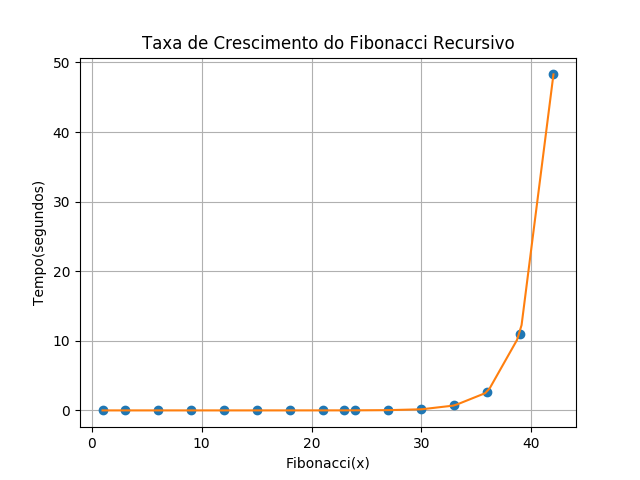
\includegraphics[width=\linewidth]{../fibonacci_recursivo.png}
\caption{Fibonacci Recursivo}
\end{minipage}
%---------------------------------------------
\hfill
%-------------SEGUNDA FIGURA------------------
\begin{minipage}[b]{0.45\linewidth}
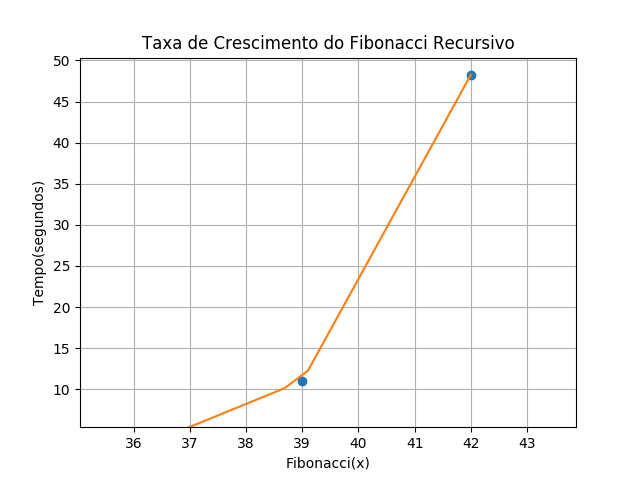
\includegraphics[width=\linewidth]{../fibonacci_recursivo_zoom.png}
\caption{Ampliado num Intervalo}
\end{minipage}
%--------------------------------------------
\end{figure}
%--------
\newpage

{\Large\bf Fibonacci Iterativo}\\

Sabendo que a complexidade do Fibonacci Interativo é $O(n)$, onde este se comporta como uma função linear, é facil vizualizar que seu custo computacional é muito mais leve do que uma função exponencial. 

Olhando para o gráfico, podemos ver que os valores de $n$ são muito maiores do que os valores utilizado no Fibonacci Recursivo, e este algorimo retorna o valor desejado praticamente instantaneamente. Se tivesse testado esses valores de $n$ no Fibonacci Recursivo, além de muito processamento exigido, poderia demorar horas, quem sabe dias para retornar o resultado desejado.


%----------AMBIENTE DE FIGURA-----------------
\begin{figure}[h]
\centering
%------------PRIMEIRA FIGURA------------------
\begin{minipage}[b]{0.45\linewidth}
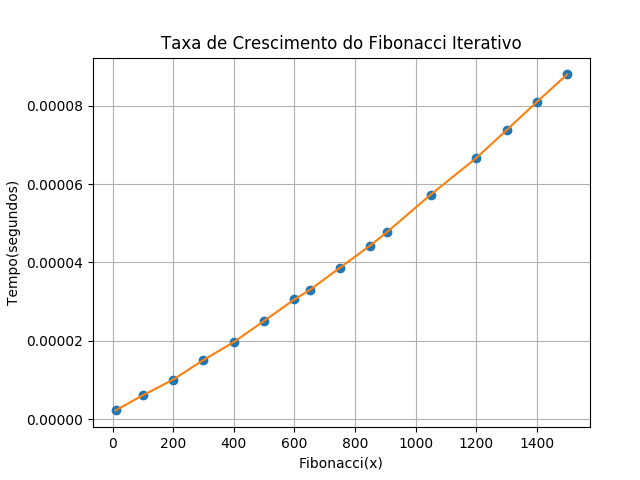
\includegraphics[width=\linewidth]{../fibonacci_iterativo.png}
\caption{Fibonacci Iterativo}
\end{minipage}
%---------------------------------------------
\hfill
%-------------SEGUNDA FIGURA------------------
\begin{minipage}[b]{0.45\linewidth}
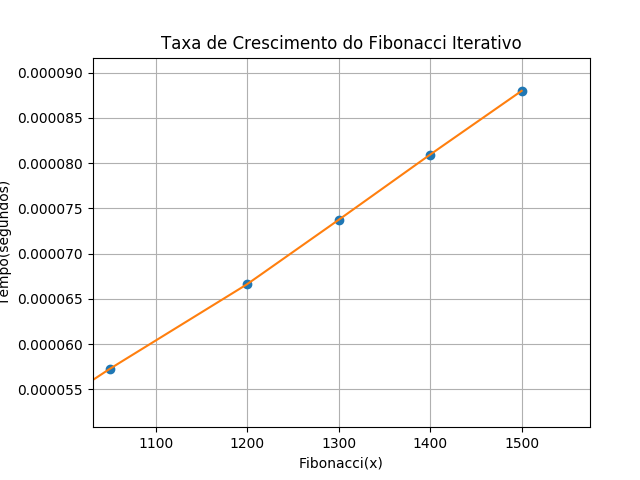
\includegraphics[width=\linewidth]{../fibonacci_iterativo_zoom.png}
\caption{Ampliado num Intervalo}
\end{minipage}
%--------------------------------------------
\end{figure} 
%--------
\newpage

\section{Conclusão}
%{\Large\bf Conclusão}\\

Portanto, é possível concluir que, para um dado problema, quanto menor possível for a complexidade para resolução do mesmo, melhor. É claro que, este é um exemplo simples e muito conhecido na computação, porém, é muito interessante para estudantes da computação que ainda não tem o conhecimento de Análise Assintótica e não sabem o que é e como se comporta a complexidade de um algoritmo a leitura deste trabalho, pois provavelmente a maioria dos alunos dos cursos de computação já escreveram um programa para mostrar a {\it Sequência de Fibonacci}, então seria um exemplo de fácil compreensão.

Existe algoritmos melhores para retornar o {\it n-ésimo} número desejado desta sequência em $O(logn)$. Porém, este foi somente um trabalho para comparar estes dois algoritmos considerando que eu já deveria realizar a Analíse Assintótica de cada um como trabalho proposto pelo professor ministrante da disciplina. 

Abaixo estão as figuras lado a lado dos dois algoritmos comparados, ampliadas num intervalo para a melhor vizualização e comparação de tempo em relação ao {\it n-ésimo} termo da sequência.

%----------AMBIENTE DE FIGURA-----------------
\begin{figure}[h]
\centering
%------------PRIMEIRA FIGURA------------------
\begin{minipage}[b]{0.45\linewidth}
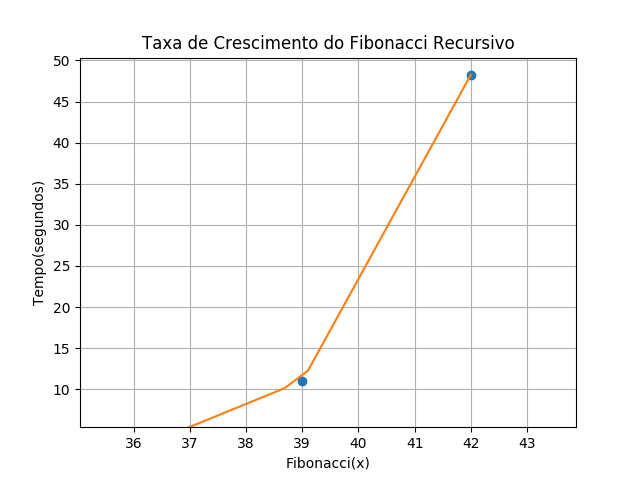
\includegraphics[width=\linewidth]{../fibonacci_recursivo_zoom.png}
\caption{\scriptsize Fibonacci Recursivo Ampliado}
\end{minipage}
%---------------------------------------------
\hfill
%-------------SEGUNDA FIGURA------------------
\begin{minipage}[b]{0.45\linewidth}
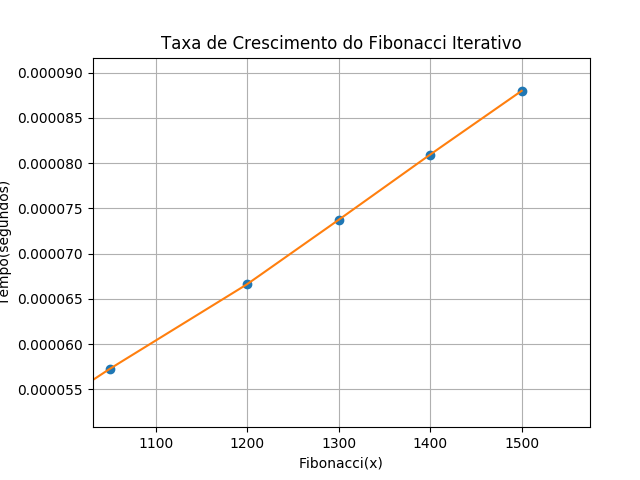
\includegraphics[width=\linewidth]{../fibonacci_iterativo_zoom.png}
\caption{\scriptsize Fibonacci Iterativo Ampliado}
\end{minipage}
%--------------------------------------------
\end{figure} 
%--------

\end{document}